\documentclass[border=3pt,tikz]{standalone}
\usepackage{amsmath}
\usetikzlibrary{arrows}
\usetikzlibrary{positioning}
\usetikzlibrary{calc}
\usetikzlibrary{arrows.meta}
\usetikzlibrary{decorations.pathreplacing}
\begin{document}
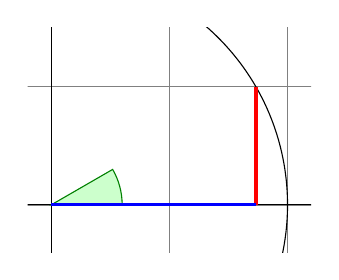
\begin{tikzpicture}[scale=3]
    \clip (-0.1,-0.2) rectangle (1.1,0.75);
    \draw[step=.5cm,gray,very thin] (-1.4,-1.4) grid (1.4,1.4);
    \draw (-1.5,0) -- (1.5,0);
    \draw (0,-1.5) -- (0,1.5);
    \draw (0,0) circle (1cm);
    \filldraw[fill=green!20,draw=green!50!black] (0,0) -- (3mm,0mm) arc
    (0:30:3mm) -- cycle;
    \draw[red,very thick]  (30:1cm) -- +(0,-0.5);
    \draw[blue,very thick] (30:1cm) ++(0,-0.5) -- (0,0);
  \end{tikzpicture}
\end{document}